% =========================================================
% ПРЕДЛОГ ТЕКСТА ЗА ПОГЛАВЉЕ 2 „Визуелна одометрија"
%
% Самостални документ са истом преамбулом као main.tex, да би могао
% да се компајлира одвојено:   latexmk -xelatex suggestion.tex
% Тело поглавља (од \section{Визуелна одометрија} до \newpage) може
% директно да се пресели у main.tex уместо постојећег TODO дела.
%
% Слике су у figures/draft/ и исечене су из оригиналних радова
% (видети коментаре изнад сваке слике и plan-poglavlje-2.md).
% Постојеће потпоглавље „Окружење" из main.tex није поновљено овде.
% =========================================================
\documentclass[12pt]{article}

\usepackage{fontspec}
\setmainfont{Times New Roman}
\usepackage{polyglossia}
\setdefaultlanguage{serbian}
\newfontfamily\cyrillicfont{Times New Roman}
\newfontfamily\cyrillicfonttt{Times New Roman}

\usepackage[a4paper, top=2cm, bottom=2cm, left=2.5cm, right=2cm, heightrounded]{geometry}

\usepackage{setspace}
\setstretch{1.15}
\usepackage{indentfirst}
\setlength{\parindent}{1.25cm}
\setlength{\parskip}{0pt}

\usepackage{amsmath, amssymb, amsthm}
\usepackage{mathrsfs}

\usepackage{graphicx}
\usepackage{float}
\graphicspath{{figures/}}

\usepackage{caption}
\captionsetup{labelsep=space}
\captionsetup[table]{justification=raggedright, singlelinecheck=false}

\usepackage{chngcntr}
\counterwithin{figure}{section}
\counterwithin{table}{section}
\counterwithin{equation}{section}

\usepackage[shortlabels]{enumitem}
\usepackage{xurl}
\usepackage{hyperref}
\hypersetup{colorlinks=true, linkcolor=black, urlcolor=blue, breaklinks=true}

\usepackage[backend=biber, style=numeric, sorting=none]{biblatex}
\addbibresource{literatura.bib}

\usepackage{comment}
\usepackage{multirow}

\begin{document}
% Да би нумерација била 2.x као у main.tex:
\setcounter{section}{1}

\section{Визуелна одометрија}

Визуелна одометрија (ВО) је поступак инкременталне процене положаја и
оријентације камере на основу промена у сликама које изазива њено кретање.
Термин је увео Нистер 2004. године по аналогији са одометријом са точкова:
као што се код одометрије са точкова положај добија интеграцијом прираштаја
углова точкова, тако се код ВО положај добија надовезивањем релативних
трансформација процењених између узастопних слика
\cite{nister2004visual, scaramuzza2011visual}. ВО је посебан случај
реконструкције структуре из кретања (\textit{Structure from Motion, SfM}),
која из скупа слика истовремено реконструише и кретање камере и тродимензионалну
структуру сцене. За разлику од општег \textit{SfM} проблема, ВО обрађује слике
секвенцијално, у реалном времену, и тежи локалној конзистентности путање, а не
глобалној оптимизацији целокупне реконструкције \cite{scaramuzza2011visual}.

ВО треба разликовати и од симултане локализације и мапирања (\textit{Simultaneous
Localization and Mapping, SLAM}). Циљ \textit{SLAM} система је изградња глобално
конзистентне мапе окружења и локализација у њој, што подразумева препознавање
претходно посећених места и затварање петљи. Систем ВО, са друге стране,
користи искључиво краткорочне информације: делове окружења прати само док су у
видном пољу и након тога их заборавља, због чега се грешка процене нагомилава
(дрифт) чак и када се камера креће кроз исти простор \cite{campos2021orbslam3}.
ВО представља основни градивни блок већине \textit{SLAM} система, па се
разлика између њих у новијим системима све више губи. У овом раду се под
успешношћу ВО подразумева тачност процењене путање у односу на референтну, без
обзира на то да ли алгоритам поседује могућност локализације.

Као и код одометрије са точкова, грешка ВО се нагомилава са пређеним путем, али
је њен извор другачији. Одометрија са точкова је осетљива на проклизавање и на
неидеалну геометрију робота, док на ВО утиче искључиво изглед окружења и начин
на који је оно забележено камером. Да би ВО могла да процени кретање, потребно
је да буду испуњени следећи услови \cite{scaramuzza2011visual}:
\begin{itemize}
	\item довољна осветљеност сцене, како би слика била оштра и добро
	      контрастна при кратком времену експозиције (видети
	      поглавље~\ref{sec:kamera}),
	\item статична сцена, јер се претпоставља да су све промене у слици
	      искључиво последица кретања камере, па покретни објекти представљају
	      сметњу,
	\item довољно текстуре, односно области са изразитим градијентом
	      интензитета на основу којих могу да се издвоје и прате
	      карактеристичне тачке и
	\item довољно преклапање узастопних слика, како би иста тачка сцене била
	      видљива у више слика; при великим брзинама и брзим ротацијама
	      преклапање опада.
\end{itemize}

Процена дубине сцене представља основу свих геометријских алгоритама ВО. У
случају стерео ВО, дубина се рачуна на основу пиксела који се подударају у
сликама леве и десне камере. На основу разлике њиховог положаја у две слике
(диспаритета), познатог растојања између камера (базне дистанце) и унутрашњих
параметара камера, положај тачке у простору се одређује према
\eqref{eq:stereo-dubina} \cite{kostavelis2016stereo}.
\begin{equation}
	\begin{bmatrix} x & y & z \end{bmatrix}
	= \begin{bmatrix} \dfrac{x_c \cdot z}{f} & \dfrac{y_c \cdot z}{f} & \dfrac{b \cdot f}{d} \end{bmatrix}
	\label{eq:stereo-dubina}
\end{equation}
У изразу \eqref{eq:stereo-dubina} са $x$, $y$ и $z$ је означен положај тачке у
координатном систему камере, $x_c$ и $y_c$ су координате пиксела у слици, $b$
је базна дистанца, $d$ је диспаритет, а $f$ је жижна даљина изражена у
пикселима. Тачност овако процењене дубине опада са квадратом удаљености, па се
у случају тачака које су много даље од базне дистанце стерео ВО своди на
случај монокуларне ВО \cite{scaramuzza2011visual}.

Монокуларна ВО не може директно да измери дубину. Уместо стерео пара, користи
се временски пар слика: тачка сцене се посматра из два различита положаја
камере, а њена дубина се реконструише триангулацијом на основу кореспонденције
у узастепним сликама. Релативно кретање између два положаја се притом
одређује из истих кореспонденција, помоћу епиполарне геометрије, тако да се
кретање и структура процењују истовремено. Пошто не постоји податак као што је
базна дистанца, на основу којег би се одредила апсолутна скала, монокуларна ВО
може да процени транслацију само до фактора скале \cite{scaramuzza2011visual}.
Скала се на почетку рада бира произвољно и затим се преноси кроз секвенцу, али
се преносом накупља и грешка скале (\textit{scale drift}). Због тога процењена
путања пре евалуације мора да се скалира према референтној, што је описано у
поглављу~\ref{sec:poravnanje}. Из истог разлога, чиста ротација око оптичког
центра представља дегенерисан случај: без транслације нема паралаксе, па дубина
нових тачака не може да се триангулише. Ово ограничење је од значаја за
секвенце коришћене у овом раду, које садрже ротације око центра робота, при
чему се камера налази изнад центра ротације.

Ток обраде ВО засноване на карактеристичним тачкама је приказан на
слици~\ref{fig:vo-pipeline}. У свакој слици се најпре детектују карактеристичне
тачке, које се затим упарују са тачкама из претходних слика или прате кроз
секвенцу. На основу кореспонденција се процењује релативно кретање камере, а
на крају се процена кретања и положаја тачака поправља локалном оптимизацијом
над више последњих слика \cite{scaramuzza2011visual, Francani2025}. Због
рачунске сложености, оптимизација се не врши над свим сликама, већ само над
подскупом који се назива кључне слике (\textit{keyframes}). Кључна слика се
бира када се камера довољно удаљи од претходне кључне слике, тако да
триангулација нових тачака буде добро условљена.

% Слика: TSformer-VO рад, Fig. 1.
% Алтернатива: нацртати сопствену верзију у draw.io са ћириличним натписима.
\begin{figure}[H]
	\centering
	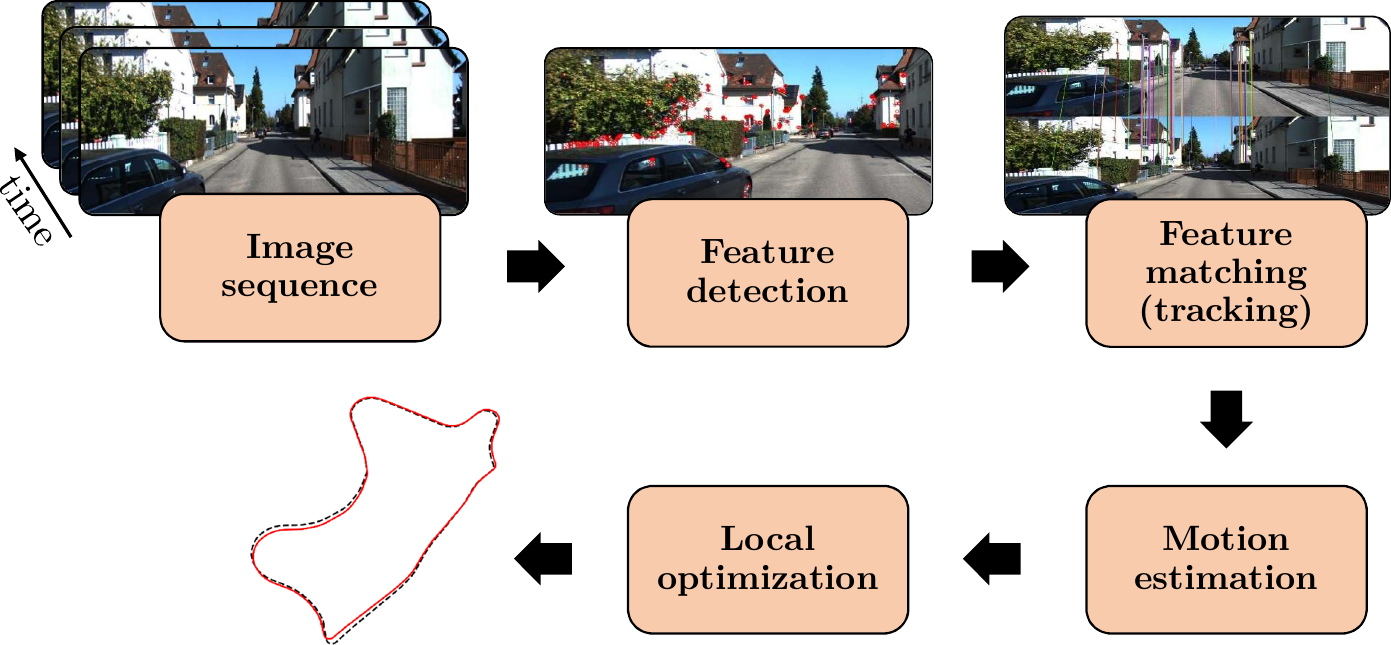
\includegraphics[width=13cm]{figures/draft/vo-pipeline-traditional.png}
	\caption{Ток обраде визуелне одометрије засноване на карактеристичним тачкама (преузето из \cite{Francani2025})}
	\label{fig:vo-pipeline}
\end{figure}

Два критеријума оптимизације се појављују у свим геометријским методама. Први
је репројекциона грешка, дата у \eqref{eq:reproj}, која представља растојање у
слици између детектоване карактеристичне тачке $\mathbf{u}_i$ и пројекције
одговарајуће 3Д тачке $\mathbf{p}_i$ при процењеној пози камере $\mathbf{T}$,
где $\pi(\cdot)$ означава пројекциони модел камере одређен унутрашњим
параметрима из поглавља~\ref{sec:kalibracija}.
\begin{equation}
	\delta \mathbf{u}_i = \mathbf{u}_i - \pi\left(\mathbf{T} \cdot \mathbf{p}_i\right)
	\label{eq:reproj}
\end{equation}
Други је фотометријска грешка, дата у \eqref{eq:fotometrijska}, која представља
разлику интензитета између пиксела $\mathbf{u}$ у претходној слици $I_{k-1}$ и
пиксела у тренутној слици $I_k$ у који се тачка са дубином $d_{\mathbf{u}}$
пресликава при релативној трансформацији $\mathbf{T}$, где је $\pi^{-1}$
инверзна пројекција \cite{forster2014svo}.
\begin{equation}
	\delta I\left(\mathbf{T}, \mathbf{u}\right)
	= I_k\Big(\pi\big(\mathbf{T} \cdot \pi^{-1}(\mathbf{u}, d_{\mathbf{u}})\big)\Big) - I_{k-1}(\mathbf{u})
	\label{eq:fotometrijska}
\end{equation}

На основу критеријума који минимизују, методе ВО се деле на геометријске и на
методе засноване на дубоком учењу, а геометријске даље на методе засноване на
карактеристичним тачкама и директне методе \cite{duan2019dlvslam}. Методе
засноване на карактеристичним тачкама експлицитно детектују и упарују
карактеристике помоћу дескриптора и минимизују репројекциону грешку
\eqref{eq:reproj}. Њихова предност је робусност на велика померања између
слика, а недостатак зависност од прагова детекције, потреба за робусним
одбацивањем погрешних кореспонденција и ограничена прецизност детектора
\cite{forster2014svo}. Директне методе не упарују дескрипторе, већ кретање и
структуру процењују непосредно из интензитета пиксела минимизацијом
фотометријске грешке \eqref{eq:fotometrijska}. Оне постижу субпикселску
прецизност и робусније су у сценама са мало текстуре, али претпостављају мала
померања између слика и константну осветљеност \cite{engel2017direct}. Методе
засноване на дубоком учењу могу да замене поједине кораке геометријског тока
обраде (хибридне методе) или да процењују позу камере из слика без иједног
геометријског модула (\textit{end-to-end} методе) \cite{Francani2025}. У овом
раду су анализирани представници сваког од та три типа метода:
\textit{SVO} као представник директних метода, \textit{ORB-SLAM3} као
представник метода заснованих на карактеристичним тачкама и
\textit{TSformer-VO} као представник метода заснованих на дубоком учењу.

\subsection{\textit{SVO}}
\textit{SVO} (\textit{Semi-Direct Visual Odometry}) је алгоритам монокуларне ВО
развијен за процену стања микро летелица, где су ограничени рачунски ресурси и
потребна је висока учестаност процене \cite{forster2014svo}. Алгоритам користи
кореспонденцију карактеристика, али с обзиром на то да она представља
имплицитан резултат директне процене кретања, а не резултат експлицитног
издвајања и упаривања карактеристика, \textit{SVO} је издвојен као представник
директних метода ВО. Издвајање карактеристика се врши само када се изабере нова
кључна слика, ради иницијализације нових 3Д тачака. Предност таквог приступа је
прескакање рачунски захтевног процеса екстракције карактеристика у сваком
фрејму, док се захваљујући директном поравнавању постиже субпикселска
прецизност кореспонденција. Чим се заврши кореспонденција карактеристика и
процена иницијалне позе камере, алгоритам наставља са коришћењем само
претходно иницијализованих 3Д тачака. За разлику од ранијих
директних метода, које су пратиле мали број великих равних површи,
\textit{SVO} прати стотине малих делова слике (\textit{patch}) величине
$4 \times 4$ пиксела, чиме се повећава робусност и избегава потреба за проценом
нормала површи \cite{forster2014svo}.

Структура алгоритма је приказана на слици~\ref{fig:svo-pipeline}. Алгоритам је,
по узору на \textit{PTAM} \cite{klein2007ptam}, подељен у две паралелне нити.
Нит за процену кретања обрађује сваку нову слику и процењује њену позу у односу
на мапу, док нит за мапирање проширује мапу новим 3Д тачкама и није везана за
рад у реалном времену.

% Слика: SVO 2014 рад, Fig. 1 (tracking and mapping pipeline).
\begin{figure}[H]
	\centering
	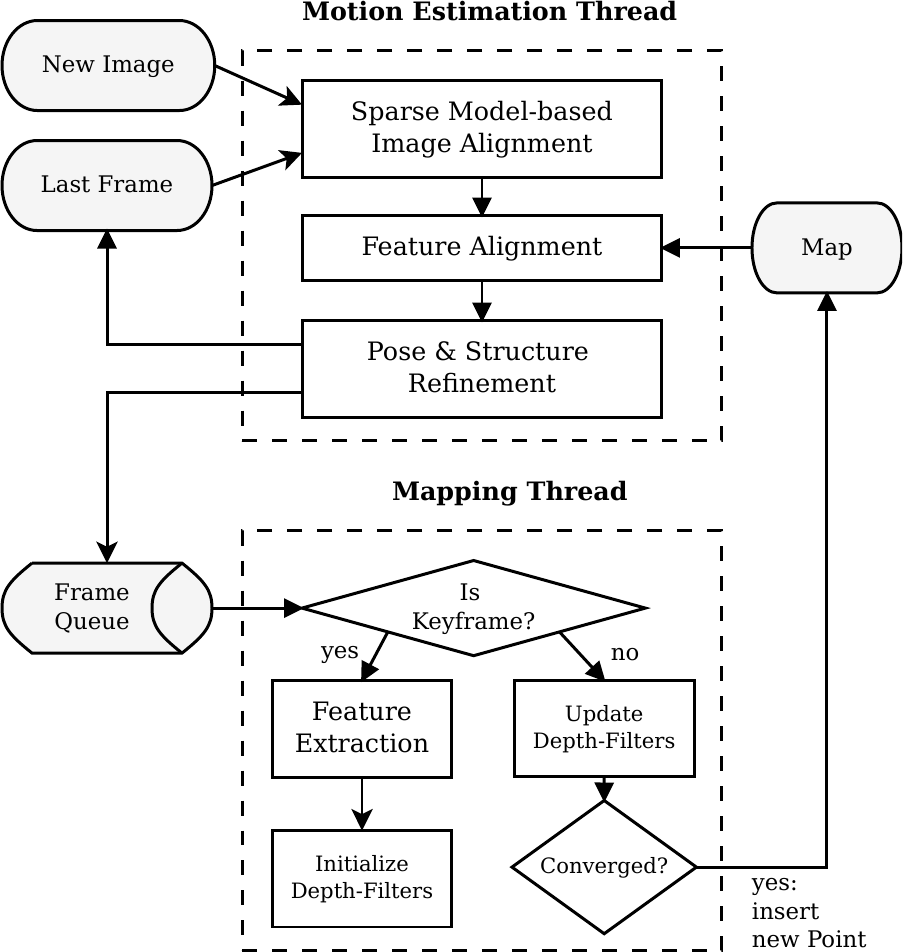
\includegraphics[width=10cm]{figures/draft/svo-pipeline.png}
	\caption{Структура алгоритма \textit{SVO}: нит за процену кретања и нит за мапирање (преузето из \cite{forster2014svo})}
	\label{fig:svo-pipeline}
\end{figure}

Процена кретања се састоји од три корака, који су илустровани на
слици~\ref{fig:svo-koraci}. У првом кораку, ретком поравнавању слике заснованом
на моделу (\textit{sparse model-based image alignment}), тражи се релативна
трансформација $\mathbf{T}_{k,k-1}$ између претходне и тренутне слике која
минимизује збир квадрата фотометријских грешака \eqref{eq:fotometrijska} по
свим деловима слике око карактеристичних тачака са познатом дубином.
Задатак се решава итеративно Гаус-Њутновим поступком, при чему се
трансформација параметризује минималном репрезентацијом у Лијевој алгебри
$\mathfrak{se}(3)$. Користи се инверзна композициона формулација, у којој се
Јакобијан рачуна над претходном сликом и остаје константан кроз све итерације,
што значајно убрзава оптимизацију. Да би се обухватила већа померања, поступак
се примењује од најгрубљег ка финијим нивоима пирамиде слике са пет нивоа
\cite{forster2014svo}.

У другом кораку, поравнавању карактеристика (\textit{feature alignment}), све
3Д тачке мапе видљиве из процењене позе се пројектују у тренутну слику, чиме се
добија почетна процена положаја карактеристика $\mathbf{u}'_i$. Због
непрецизности 3Д тачака и позе, положај сваког дела слике се затим појединачно
поправља минимизацијом фотометријске грешке у односу на референтни део из
кључне слике која ту тачку посматра под најсличнијим углом. Пошто је кључна
слика по правилу удаљенија од претходне слике, у овом кораку се користе већи
делови слике ($8 \times 8$ пиксела) на које се пре поређења примењује афина
трансформација. Овај корак представља релаксацију: сваки део
слике се помера независно, чиме се нарушавају епиполарна ограничења, али се
постиже већа корелација између делова слика и кореспонденција са субпикселском
прецизношћу \cite{forster2014svo}.

У трећем кораку, поправљању позе и структуре (\textit{pose and structure
refinement}), поново се оптимизује поза камере у односу на светски координатни
систем, овај пут минимизацијом збира квадрата репројекционих грешака
\eqref{eq:reproj} које су настале у претходном кораку.
Ово је класичан проблем оптимизације само кретања (\textit{motion-only bundle
adjustment}). Након позе се на исти начин поправљају и положаји посматраних 3Д
тачака, а опционо се врши и локална оптимизација над свим блиским кључним
сликама заједно са тачкама. Аутори наводе да сам први корак даје позу веома
близу коначној, а да поравнавање у односу на кључне слике и мапу, уместо само у
односу на претходну слику, значајно смањује дрифт \cite{forster2014svo}.

% Слика: SVO 2014 рад, Fig. 2, 3 и 4 (три корака процене кретања).
% Ако је превише простора, оставити само Fig. 2 (image alignment).
\begin{figure}[H]
	\centering
	\begin{minipage}[b]{0.31\textwidth}
		\centering
		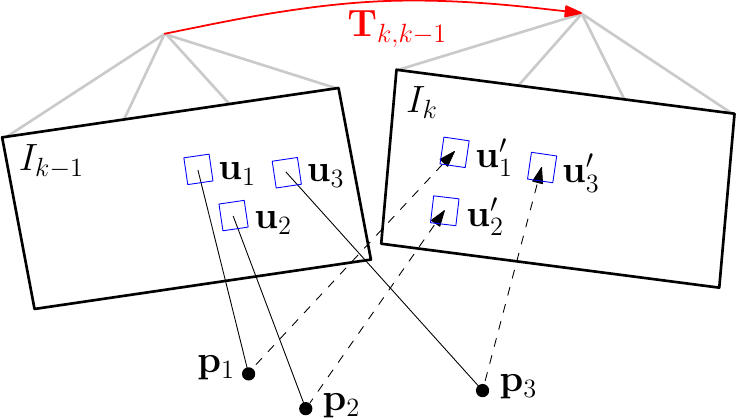
\includegraphics[width=\textwidth]{figures/draft/svo-fig2-image-alignment.png}\\
		(а)
	\end{minipage}
	\hfill
	\begin{minipage}[b]{0.33\textwidth}
		\centering
		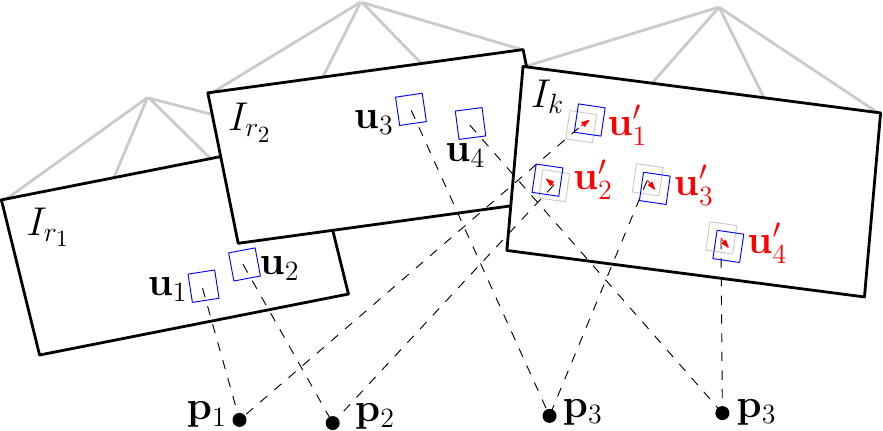
\includegraphics[width=\textwidth]{figures/draft/svo-fig3-feature-alignment.png}\\
		(б)
	\end{minipage}
	\hfill
	\begin{minipage}[b]{0.33\textwidth}
		\centering
		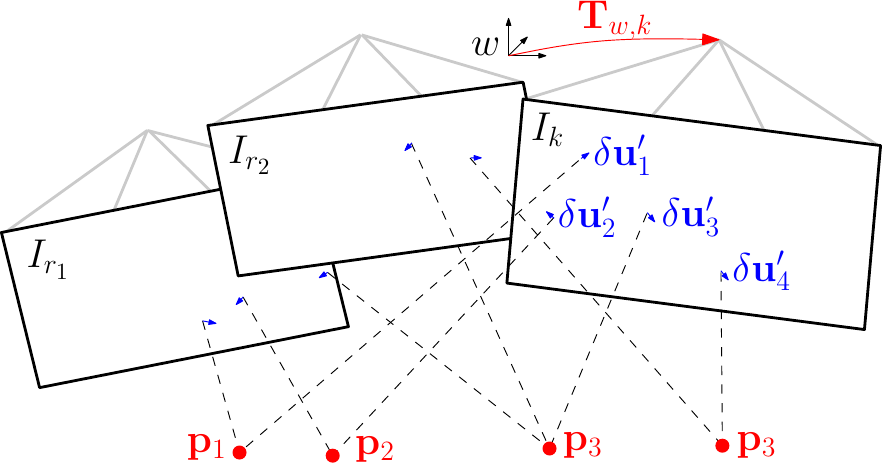
\includegraphics[width=\textwidth]{figures/draft/svo-fig4-refinement.png}\\
		(в)
	\end{minipage}
	\caption{Три корака процене кретања у \textit{SVO} алгоритму: (а) ретко поравнавање слике, (б) поравнавање карактеристика и (в) поправљање позе и структуре (преузето из \cite{forster2014svo})}
	\label{fig:svo-koraci}
\end{figure}

Нит за мапирање процењује дубину карактеристичних тачака чије 3Д тачке још
нису познате. Уместо да се тачка триангулише из само два погледа, дубина сваке
карактеристике се моделује расподелом вероватноће, коју одржава Бајесов филтар
дубине. Филтар се иницијализује са великом неодређеношћу и средњом вредношћу
једнаком просечној дубини сцене у референтној кључној слици. За сваку наредну
слику се дуж епиполарне линије тражи део слике са највећом корелацијом у односу
на референтни, а из његовог положаја се триангулацијом добија мерење дубине
$\tilde{d}$. Мерење се моделује мешавином Гаусове и униформне расподеле, дате у
\eqref{eq:svo-depth}, где $\rho$ представља вероватноћу да је мерење исправно,
$\tau^2$ варијансу исправног мерења, а $[d_{\min}, d_{\max}]$ интервал у којем
се јављају погрешна мерења \cite{forster2014svo}.
\begin{equation}
	p\left(\tilde{d} \mid d, \rho\right)
	= \rho \, \mathcal{N}\!\left(\tilde{d} \mid d, \tau^2\right)
	+ \left(1 - \rho\right) \mathcal{U}\!\left(\tilde{d} \mid d_{\min}, d_{\max}\right)
	\label{eq:svo-depth}
\end{equation}
Претрага дуж епиполарне линије је ограничена на две стандардне девијације око
тренутне процене, а дубина се представља у инверзном облику ради стабилности
при великим удаљеностима. Тек када варијанса филтра постане довољно мала, 3Д
тачка се уноси у мапу и одмах користи за процену кретања. Пошто свака тачка
пролази кроз више мерења пре него што се прихвати, мапа садржи веома мало
погрешних тачака, што је главни разлог робусности алгоритма у сценама са
понављајућом текстуром \cite{forster2014svo}.

Алгоритам се иницијализује из прве две кључне слике под претпоставком локално
равне сцене, проценом хомографије, из које се триангулише почетна мапа. Нова
кључна слика се бира када растојање тренутне слике од свих кључних слика пређе
12\,\% просечне дубине сцене; у мапи се чува ограничен број кључних слика, а
најудаљенија се уклања. Карактеристике се детектују као \textit{FAST} углови на
свим нивоима пирамиде, при чему се слика дели на мрежу ћелија величине
$30 \times 30$ пиксела и у свакој ћелији задржава само угао са највећим
\textit{Shi-Tomasi} скором, чиме се обезбеђује равномеран распоред
карактеристика \cite{forster2014svo}. Аутори су на снимку са летелице
пријавили релативну грешку позиције од $0{,}0059\,\mathrm{m/s}$ у односу на
$0{,}0164\,\mathrm{m/s}$ за \textit{PTAM}, при учестаности од преко 300 слика
у секунди на лаптопу и 55 слика у секунди на уграђеном рачунару
\cite{forster2014svo}.

У овом раду је коришћена отворена имплементација \textit{SVO Pro}
\cite{svo_pro_open}, која реализује проширену верзију алгоритма
\cite{forster2017svo}. У односу на изворни алгоритам, проширена верзија поред
углова прати и ивичне сегменте (\textit{edgelets}), код којих се поравнавање
врши само дуж нормале ивице, подржава уношење претходног знања о кретању у
корак поравнавања слике, општије моделе камере, као и рад са више камера
\cite{forster2017svo}. Имплементација додатно нуди оптимизациони систем са
клизним прозором заснован на \textit{Ceres} библиотеци, спрегу са инерцијалним
сензором и затварање петљи помоћу \textit{DBoW2}. У овом раду је коришћен
искључиво монокуларни предњи део система, односно чиста ВО без инерцијалног
сензора, оптимизације у позадини и затварања петљи. Због тога \textit{SVO} овде
представља алгоритам који користи само краткорочне информације: скала се
преноси кроз секвенцу без могућности корекције, а при ротацији око центра
робота, због изостанка паралаксе, филтри дубине не могу да конвергирају и не
бирају се нове кључне слике.

\subsection{\textit{ORB-SLAM3}}
\textit{ORB-SLAM3} је систем за визуелни и визуелно-инерцијални \textit{SLAM}
заснован на карактеристичним тачкама, који подржава монокуларне, стерео и
\textit{RGB-D} камере \cite{campos2021orbslam3}. Систем је наследник
\textit{ORB-SLAM} \cite{murartal2015orbslam} и \textit{ORB-SLAM2}
\cite{murartal2017orbslam2}, од којих преузима основну архитектуру. Аутори
разликују три нивоа повезивања података. Краткорочно повезивање упарује
елементе мапе из последњих неколико секунди и једини је ниво који користе
системи ВО. Средњорочно повезивање упарује тренутну слику са елементима мапе
који су близу камере, а чија је накупљена грешка још увек мала, чиме се дрифт
своди на нулу док се систем креће кроз већ мапирано подручје. Дугорочно
повезивање, засновано на препознавању места, упарује тренутну слику са
претходно посећеним подручјем без обзира на накупљени дрифт и омогућава
затварање петље, поновну локализацију након губитка праћења и спајање мапа
\cite{campos2021orbslam3}. \textit{ORB-SLAM3} је изабран не само као
представник метода заснованих на карактеристичним тачкама, већ и како би се
испитало колико локализација доприноси успешности ВО у поређењу са алгоритмима
који користе само краткорочне информације.

Систем у свим корацима користи \textit{ORB} карактеристике
\cite{rublee2011orb}, које комбинују \textit{FAST} детектор углова са
оријентацијом и бинарни \textit{BRIEF} дескриптор ротиран према тој
оријентацији. Карактеристике се издвајају на пирамиди слике са осам нивоа и
равномерно распоређују по мрежи ћелија, а по слици се издваја реда 1000
карактеристика. Бинарни дескриптори се упарују Хеминговим растојањем, што је
веома брзо, а исти дескриптори се користе и за препознавање места помоћу
\textit{bag-of-words} модела \textit{DBoW2} \cite{galvez2012dbow2}.

Главне компоненте система су приказане на слици~\ref{fig:orbslam3}. Систем чине
три нити које раде паралелно и структура \textit{Atlas}, која садржи скуп
раздвојених мапа. У сваком тренутку постоји једна активна мапа, у којој се
локализују долазне слике и коју нит за локално мапирање проширује, док остале
мапе остају неактивне. Систем одржава јединствену \textit{DBoW2} базу кључних
слика над свим мапама, која се користи за поновну локализацију, затварање
петљи и спајање мапа \cite{campos2021orbslam3}.

% Слика: ORB-SLAM3 рад, Fig. 1 (main system components).
\begin{figure}[H]
	\centering
	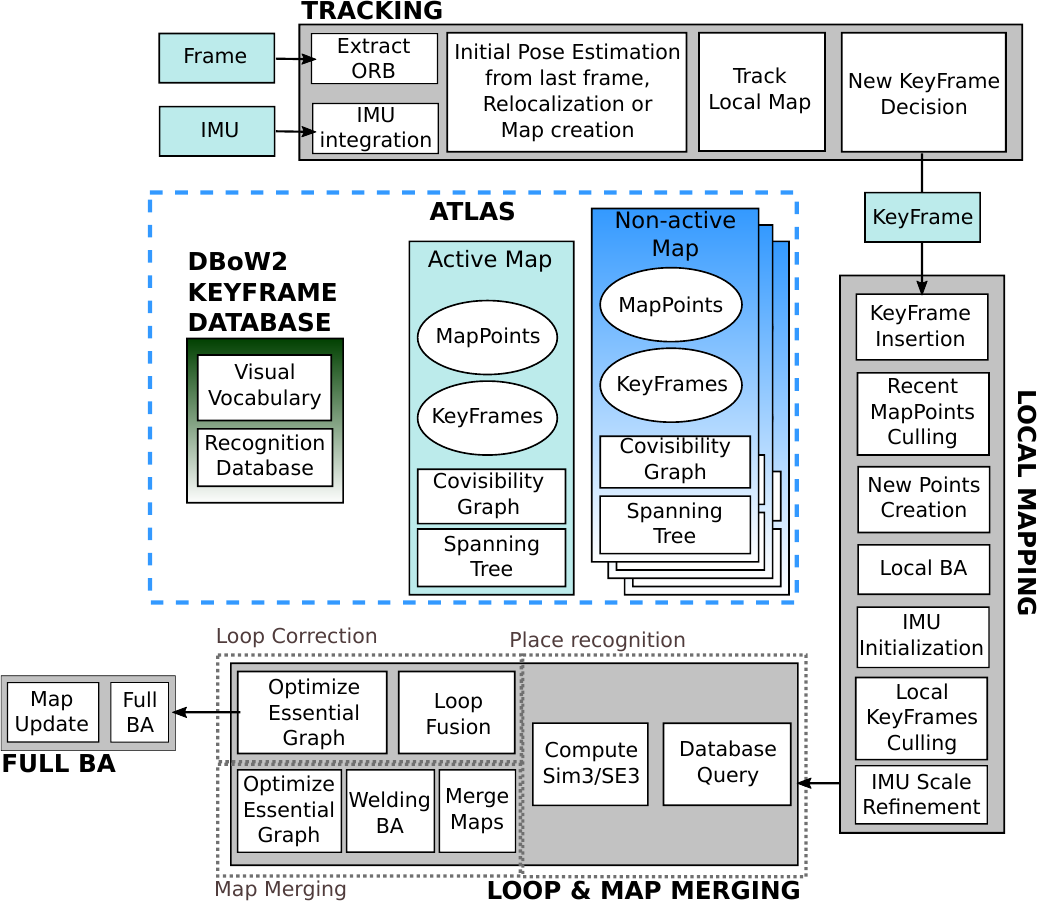
\includegraphics[width=12cm]{figures/draft/orbslam3-components.png}
	\caption{Главне компоненте система \textit{ORB-SLAM3} (преузето из \cite{campos2021orbslam3})}
	\label{fig:orbslam3}
\end{figure}

Нит за праћење обрађује сваку слику и рачуна њену позу у односу на активну мапу
минимизацијом репројекционе грешке упарених карактеристика. Почетна процена
позе се добија из модела константне брзине, а карактеристике се упарују
пројекцијом тачака мапе посматраних из претходне слике у уски прозор око
предвиђеног положаја. Затим се прате све тачке локалне мапе, коју чине кључне
слике које деле посматране тачке са тренутном сликом (ковизибилне кључне
слике), и поза се поправља оптимизацијом само кретања, односно минимизацијом
репројекционих грешака \eqref{eq:reproj} свих упарених карактеристика. За
разлику од \textit{SVO} алгоритма, који минимизује прост збир квадрата, овде се
на сваку грешку примењује Хуберова функција цене, која умањује утицај погрешних
кореспонденција \cite{murartal2015orbslam, campos2021orbslam3}.
Нит за праћење на крају одлучује да ли тренутна слика постаје кључна, што се
дешава када је од последње кључне слике прошло довољно слика и када тренутна
слика прати довољно тачака, али мањи део тачака референтне кључне слике.
Уколико се праћење изгуби, систем покушава поновну локализацију у свим мапама
структуре \textit{Atlas}: \textit{DBoW2} база враћа кандидате кључних слика, а
поза се затим рачуна \textit{PnP} алгоритмом уз \textit{RANSAC}. Уколико
локализација не успе у одређеном року, активна мапа се чува као неактивна и
започиње се нова активна мапа од почетка \cite{campos2021orbslam3}. Ово је
понашање које је уочено у резултатима из поглавља~\ref{sec:rezultati-orb}.

Нит за локално мапирање обрађује нове кључне слике: додаје их у активну мапу,
уклања недавно унете тачке које се не прате поуздано, триангулише нове тачке из
кореспонденција са ковизибилним кључним сликама, изводи локалну оптимизацију
(\textit{local bundle adjustment}) над ковизибилним кључним сликама и њиховим
тачкама и на крају уклања сувишне кључне слике чије тачке су већ посматране из
довољно других кључних слика \cite{murartal2017orbslam2}.

Нит за затварање петљи и спајање мапа се покреће при уносу сваке кључне слике и
тражи заједничка подручја између активне мапе и целе структуре \textit{Atlas}.
\textit{DBoW2} база враћа три најсличније кључне слике, за сваког кандидата се
формира локални прозор од његових ковизибилних кључних слика и тачака, а затим
се \textit{RANSAC} поступком рачуна трансформација која поравнава тачке
активне мапе са тачкама кандидата. У монокуларном случају та трансформација
припада групи сличности $\mathrm{Sim}(3)$, јер је мапа позната само до фактора
скале, па се затварањем петље исправља и дрифт скале. Хипотеза се потврђује
вођеним упаривањем и нелинеарном оптимизацијом, а за разлику од претходних
верзија, потврда се тражи у кључним сликама које су већ у мапи уместо да се
чека на три наредне кључне слике, чиме се повећава одзив препознавања места
\cite{campos2021orbslam3}. Уколико заједничко подручје припада активној мапи,
врши се корекција петље: дуплиране тачке се спајају, оптимизује се граф
кључних слика, а затим се у посебној нити покреће глобална оптимизација. Уколико
подручје припада неактивној мапи, врши се спајање мапа у прозору око упарених
кључних слика, након чега се корекција пропагира на остатак мапе оптимизацијом
графа \cite{campos2021orbslam3}.

У монокуларном режиму систем се иницијализује из две слике са довољном
паралаксом, при чему се паралелно рачунају хомографија, за случај равне сцене,
и фундаментална матрица, за случај опште сцене, а модел се бира на основу
статистичког критеријума \cite{murartal2015orbslam}. Као и код осталих
монокуларних метода, чиста ротација не омогућава триангулацију нових тачака,
што аутори експлицитно наводе као ограничење \cite{campos2021orbslam3}. Систем
ради у реалном времену са 30 до 40 слика у секунди, а на скупу података
\textit{EuRoC} у монокуларном режиму постиже средњу апсолутну грешку путање од
$0{,}041\,\mathrm{m}$, у односу на $0{,}294\,\mathrm{m}$ за \textit{SVO} и
$0{,}601\,\mathrm{m}$ за \textit{DSO}, што аутори приписују коришћењу
средњорочног и дугорочног повезивања података. Као главни разлог отказивања
аутори наводе окружења са мало текстуре, док губитак праћења при брзим
покретима ублажава могућност започињања нове мапе \cite{campos2021orbslam3}. У
овом раду је коришћена монокуларна конфигурација система без инерцијалног
сензора, са укљученим затварањем петљи и спајањем мапа.

\subsection{\textit{TSformer-VO}}
\textit{TSformer-VO} је \textit{end-to-end} метода монокуларне ВО заснована на
дубоком учењу, која проблем процене кретања посматра као задатак разумевања
видеа \cite{Francani2025}. Уместо детекције и упаривања карактеристика и
геометријских модула, модел непосредно из кратког исечка узастопних слика
регресијом процењује релативне позе камере са шест степени слободе. Модел је
заснован на архитектури \textit{TimeSformer}, која је развијена за
препознавање акција у видеу и која механизам самопажње (\textit{self-attention})
примењује истовремено дуж просторне и временске димензије
\cite{bertasius2021timesformer}. Мотивација аутора је да методе засноване на
дубоком учењу не захтевају подешавање параметара за конкретан сценарио и да
имплицитно уче скалу кретања из података за обучавање, што геометријске
монокуларне методе не могу \cite{Francani2025}.

Структура модела је приказана на слици~\ref{fig:tsformer}. Улаз чини исечак
од $N_f$ узастопних слика, $\mathbf{X} \in \mathbb{R}^{N_f \times C \times H \times W}$,
где су $C$, $H$ и $W$ број канала, висина и ширина слике. Свака слика се дели
на $N = HW/P^2$ непреклапајућих делова величине $P \times P$ пиксела, који се
развијају у векторе и линеарним пресликавањем (еквивалентним 2Д конволуцији)
уграђују у токене димензије $E_d$, по узору на \textit{ViT} архитектуру
\cite{dosovitskiy2021vit}. Сваком токену се додаје научено позиционо
уграђивање, а на почетак низа се додаје посебан класни токен (\textit{cls}), који
кроз слојеве сакупља информације са свих делова свих слика и на излазу
представља цео исечак. Низ токена пролази кроз $L_x$ блокова
\textit{Transformer} енкодера, а класни токен се на крају прослеђује излазном
вишеслојном перцептрону (\textit{MLP head}). Пошто су за једну релативну позу
потребне две узастопне слике, за исечак од $N_f$ слика излаз чини $N_f - 1$
поза, односно излазни слој има димензију $6(N_f - 1)$: три компоненте
транслације и три Ојлерова угла \cite{Francani2025}.

% Слика: TSformer-VO рад, Fig. 2 (иста слика је коришћена у зборнику као slika_2.png).
\begin{figure}[H]
	\centering
	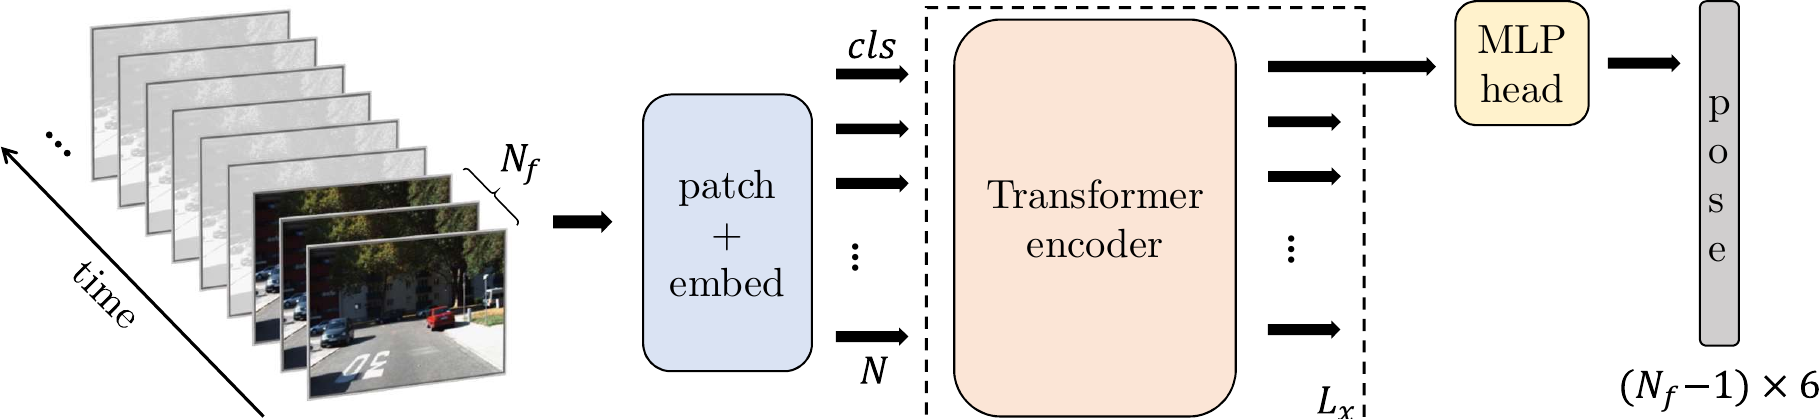
\includegraphics[width=15cm]{figures/draft/tsformer-pipeline.png}
	\caption{Структура модела \textit{TSformer-VO} (преузето из \cite{Francani2025})}
	\label{fig:tsformer}
\end{figure}

Свака слика исечка се, дакле, представља као низ токена, а модел учи односе
између токена и у простору и у времену. \textit{TimeSformer} нуди више начина
да се самопажња прошири на просторно-временски домен. Заједничка
просторно-временска самопажња повезује све парове токена из целог исечка,
што има квадратну сложеност у односу на укупан број токена. Због рачунских
ограничења у примени ВО у реалном времену, аутори су изабрали подељену
просторно-временску самопажњу (\textit{divided space-time attention}), у којој се
у сваком блоку најпре примењује временска самопажња, између токена са истим
просторним положајем у различитим сликама, а затим просторна самопажња, између
токена унутар исте слике \cite{Francani2025, bertasius2021timesformer}. Блок
енкодера је приказан на слици~\ref{fig:tsformer-enkoder}. Испред сваке од две
самопажње се налази нормализација слоја, између њих потпуно повезани слој, а на
крају блока вишеслојни перцептрон; обе самопажње и перцептрон су обухваћени
резидуалним везама \cite{Francani2025}.
Архитектура је заснована на \textit{DeiT-small} моделу, са $L_x = 12$ блокова,
$N_h = 6$ глава, димензијом уграђивања $E_d = 384$ и величином дела слике
$P = 16$ пиксела. Аутори су обучили три варијанте модела, које се разликују
само по броју слика у исечку и, последично, по димензији излазног слоја:
\textit{TSformer-VO-1} са $N_f = 2$, \textit{TSformer-VO-2} са $N_f = 3$ и
\textit{TSformer-VO-3} са $N_f = 4$. Све три варијанте имају око 30,66 милиона
параметара, а време закључивања по исечку износи од 20 до 38 милисекунди
\cite{Francani2025}.

% Слика (опционо): TSformer-VO рад, Fig. 3 (блок енкодера са подељеном самопажњом).
% Ако је поглавље предугачко, ова слика може да се изостави, а текст остаје.
\begin{figure}[H]
	\centering
	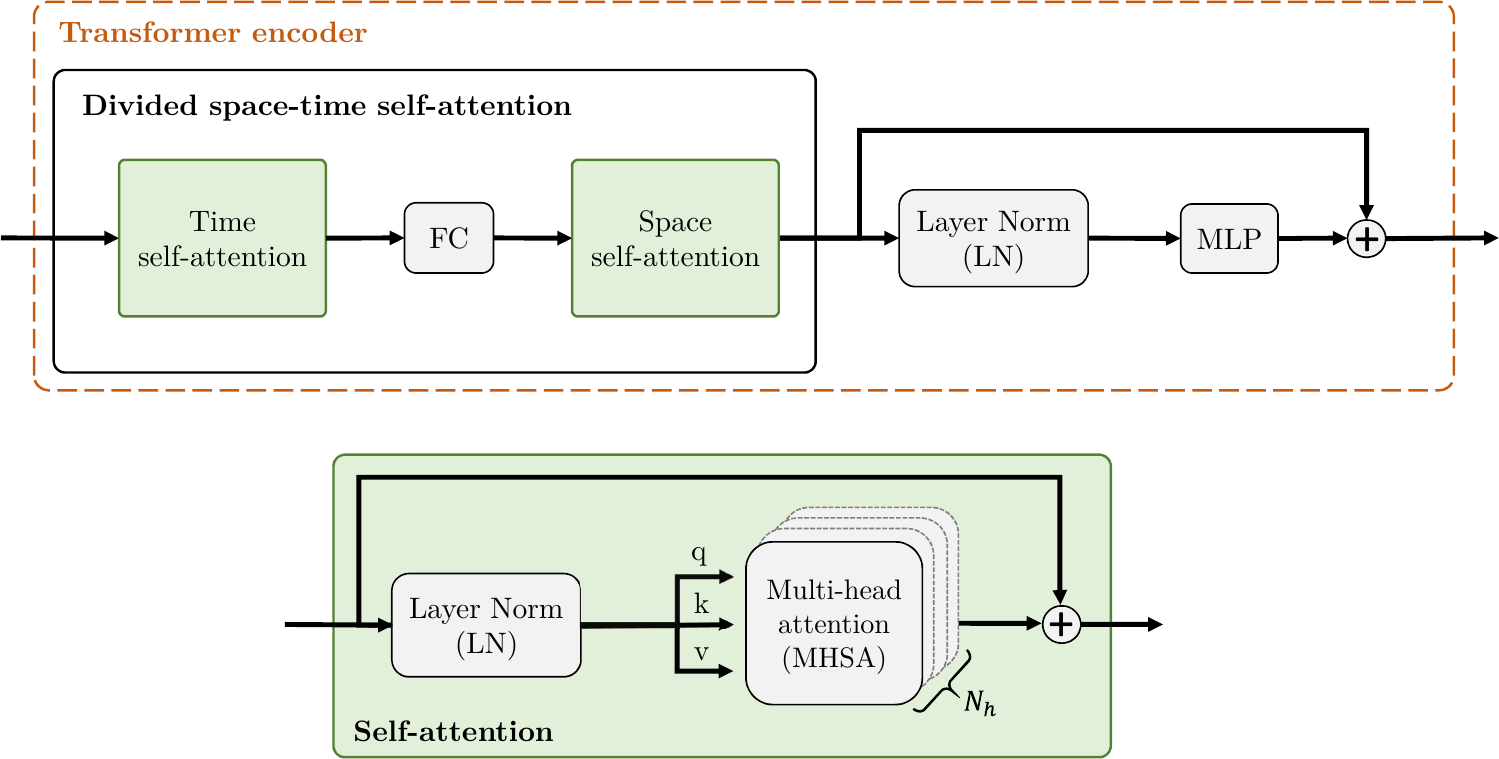
\includegraphics[width=13cm]{figures/draft/tsformer-encoder.png}
	\caption{Блок \textit{Transformer} енкодера са подељеном просторно-временском самопажњом (преузето из \cite{Francani2025})}
	\label{fig:tsformer-enkoder}
\end{figure}

Пошто модел процењује релативно кретање, референтне позе се пре обучавања
претварају из апсолутних у релативне, множењем инверзне апсолутне позе из
претходног тренутка са апсолутном позом у тренутном, а матрица ротације се
претвара у Ојлерове углове. Улазни подаци се нормализују средњом вредношћу и
стандардном девијацијом скупа за обучавање.
Модел се обучава минимизацијом средње квадратне грешке између процењених и
референтних релативних поза, дате у \eqref{eq:tsformer-loss}, где је $B_s$
величина групе (\textit{batch}), $\mathbf{y}_{i,n}$ $i$-ти елемент вектора
референтних поза $n$-тог исечка, а $\hat{\mathbf{y}}_{i,n}$ његова процена
\cite{Francani2025}.
\begin{equation}
	\mathcal{L}_{\mathrm{MSE}} = \dfrac{1}{6 B_s \left(N_f - 1\right)} \sum_{n=1}^{B_s} \sum_{i=1}^{6\left(N_f - 1\right)} \left(\mathbf{y}_{i,n} - \hat{\mathbf{y}}_{i,n}\right)^2
	\label{eq:tsformer-loss}
\end{equation}
При закључивању се исечци узимају клизним прозором са кораком од једне слике,
тако да се узастопни исечци преклапају у $N_f - 1$ слика и иста релативна поза
се процењује из више исечака. Коначна процена за сваки тренутак се добија
усредњавањем свих процена те позе, након чега се релативне позе денормализују,
Ојлерови углови враћају у матрицу ротације, а путања реконструише
надовезивањем релативних трансформација, поступком инверзним у односу на
претходну обраду \cite{Francani2025}.

Модел је обучен на скупу података \textit{KITTI} \cite{kitti_benchmark}, који
садржи снимке са возила у градској вожњи прикупљене брзином од 10 слика у
секунди. Коришћене су црно-беле слике леве камере, смањене на резолуцију
$192 \times 640$ пиксела како би димензије биле дељиве величином дела слике
$P$. За обучавање су коришћене секвенце 00, 02, 08 и 09, а за тестирање
секвенце 01, 03, 04, 05, 06, 07 и 10, по узору на \textit{DeepVO}
\cite{wang2017deepvo}. Модел је обучаван од почетка током 100 епоха
\textit{Adam} оптимизатором, при чему су аутори утврдили да претходно
обучавање на \textit{ImageNet} скупу не побољшава резултате због велике
разлике између домена \cite{Francani2025}. На тест секвенцама
\textit{TSformer-VO} је надмашио \textit{DeepVO} по већини критеријума и
постигао резултате упоредиве са \textit{ORB-SLAM3} у транслацији, док је
\textit{ORB-SLAM3} остао тачнији у ротацији. Аутори посебно наводе да модел
процењује скалу транслације без накнадног поравнавања са референтном путањом,
али и да научена скала зависи од скупа за обучавање, па за друге скупове
података може бити потребно додатно подешавање, као и да робусност модела на
унутрашња окружења и промене осветљења остаје за будућа истраживања
\cite{Francani2025}.

У овом раду су коришћене претходно обучене тежине све три варијанте модела
које су аутори објавили, без додатног обучавања на сопственом скупу података.
Слике са камере робота су, као и у изворном раду, претходно смањене на улазну
резолуцију модела. Резултати у поглављу~\ref{sec:rezultati-tsformer} су
приказани за варијанту \textit{TSformer-VO-3}.
% ПРОВЕРИТИ: вредности ATE и RPE_rot у табели резултата (2.202, 2.182, 2.187,
% 2.362 m; 0.222, 0.225, 0.319, 0.336 deg) се тачно поклапају са
% eval/results/TSformer-VO/Model1/result.txt (TSformer-VO-1), док Model3 даје
% ATE 1.846-2.023 m. Ускладити назив варијанте са табелом пре предаје.
С обзиром на то да се експериментални подаци из овог рада значајно разликују од
скупа за обучавање, како по окружењу (лабораторија уместо саобраћаја), тако и
по камери и учестаности снимања, овакво коришћење модела пре свега испитује
његову способност уопштавања на нови домен.

\newpage
\printbibliography
\end{document}
